\chapter{Approccio terapeutico al linfoma non Hodgkin}

\section{"Watch and wait"}
L’approccio terapeutico al linfoma non-Hodgkin, dipende da diversi fattori: dal sottotipo di linfoma, 
dallo stadio della malattia, dall’eventuale presenza di “sintomi B” come febbre, sudorazione notturna, 
perdita di peso superiore al 10\% negli ultimi sei mesi, ed il possibile coinvolgimento extranodale\cite{LLS}.\\
L’approccio “watch and wait” viene scelto per pazienti con linfoma indolente, che non presentano sintomi e che 
alla diagnosi mostrano un’estensione della patologia limitata. 
Si tratta di un’osservazione attenta nel corso del tempo, mediante analisi ed esami mirati.\\
Alcuni studi hanno mostrato come non ci fosse una differenza a livello di sopravvivenza tra i pazienti che venivano 
fin da subito sottoposti a trattamento rispetto a chi invece veniva osservato nel tempo; l’approccio da scegliere 
viene concordato tra il medico e il paziente, in quanto ogni caso è a sé e deve essere valutato singolarmente\cite{LLS}.\\
Per alcuni pazienti la malattia può restare stabile o progredire lentamente per molti anni, 
per altri invece può evolvere in forme aggressive di LNH che necessita pertanto di trattamento tempestivo.\\
Per pazienti con linfoma aggressivo invece si ha un approccio di polichemioterapia basata su schemi terapeutici 
che associano farmaci chemioterapici, corticosteroidi e anticorpi monoclonali. 
Per quel che riguarda la chemioterapia, sarà approfondita in un capitolo a parte.\\ 
In questo capitolo ci concentreremo su altri approcci terapeutici: 
radioterapia, immunoterapia, trapianto autologo e allogenico di cellule staminali emopoietiche.\\

\section{Radioterapia}
La radioterapia usa radiazioni ad alte dosi per distruggere le cellule cancerose o per rallentare la loro crescita, 
distruggendo il loro DNA. 
La radioterapia può essere esterna o interna, quest'ultima è detta anche brachiterapia. 
La caratteristica della radioterapia esterna è che è un trattamento localizzato, cioè rivolto alla sola parte 
del corpo interessata dal tumore. 
Per quanto riguarda la radioterapia interna, possiamo parlare di brachiterapia o di radioterapia sistemica. 
La brachiterapia è un trattamento locale, quindi di una specifica parte del corpo, in cui particelle contenenti 
radiazioni vengono immesse nel tumore o nelle sue vicinanze. 
La radioterapia sistemica è così definita perché il trattamento è immesso nel corpo per via orale, endovenosa o 
tramite iniezione e questo modo raggiunge tutti i tessuti del corpo; con questo trattamento i liquidi biologici 
come urina, saliva e sudore, risulteranno radioattivi per qualche giorno, fino a che il corpo non avrà smaltito 
tali sostanze\cite{NIH}.\\
Nel LNH, la radioterapia è usata come unico trattamento in caso di stadi di malattia molto precoci, 
altrimenti è un trattamento generalmente combinato ad altri, come la chemioterapia, nonché può essere 
coadiuvata al trapianto di cellule staminali; può essere anche impiegata per alleviare i sintomi causati da 
linfomi che interessano cervello, midollo spinale e per tumori che comprimono i nervi\cite{ACSRADIATION}.\\
È impiegata in caso di malattia bulky o dopo il trattamento di chemioterapia per prevenire le recidive. 
Prima della radioterapia il team deve pianificare il trattamento: decide la dose necessaria, bisogna assicurarsi 
che il trattamento sia rivolto principalmente alle cellule cancerose e il meno possibile alle cellule sane, 
per evitare di danneggiarle; si esegue una TC dell’area da trattare, un momento in cui è di fondamentale importanza 
mantenere una posizione ferma, in quanto essa viene registrata e sarà la posizione in cui verrà eseguita la 
radioterapia\cite{MACMILLAN}.\\
In caso di radioterapia che interessa testa e collo vengono prodotti degli immobilizzatori che aiutano a mantenere 
la postura. La durata del trattamento dipende dal tipo e dall’estensione del linfoma, il trattamento non provoca 
dolore, si sentono i rumori emessi dalla macchina e si può comunicare con il team tramite dei microfoni, da cui 
possono dare indicazioni o a cui ci si può rivolgere in caso di malessere\cite{UKRADIOTP}.\\

\subsection{Effetti collaterali della radioterapia}
Gli effetti collaterali della radioterapia dipendono dalla parte del corpo interessata dal trattamento; 
medici e infermieri informano il paziente sulla possibilità che diversi sintomi possono presentarsi, la gravità e 
la durata del sintomo variano da persona a persona. 
Il paziente viene informato su come gestire tali sintomi, è importante informare il medico per quanto riguarda la 
loro comparsa ed avvisare se persistono o peggiorano. Effetti a lungo termine sono rari e dipendono dalla parte 
del corpo trattata\cite{MACMILLAN}.\\
La radioterapia per il LNH può provocare, nel breve termine, arrossamento e dolore della pelle, a livello dell’area 
trattata; la pelle può sembrare una scottatura solare, può dare prurito e formare vescicole; questi cambiamenti possono
presentarsi fino a 2-4 settimane dopo la fine del trattamento. Bisogna seguire alcuni accorgimenti di skin care 
dell’area trattata: non usare borotalco, quando ci si lava usare acqua e sapone senza strofinare vigorosamente, 
asciugare tamponando; non usare profumi, non eseguire ceretta; si può usare il deodorante normalmente, a meno che 
la pelle non sia danneggiata; gli uomini possono usare rasoi elettrici; non applicare medicazioni; si può eseguire 
lo shampoo, ma non asciugare i capelli con l’asciugacapelli, se il trattamento interessa la testa.\\ 
Durante il trattamento di radioterapia, indossare indumenti comodi, prodotti con fibre naturali, evitare i reggiseni; 
fare attenzione all’esposizione al sole fino ad un anno dopo la fine della radioterapia, usando sempre la crema 
solare ad alta protezione\cite{UKRADIOTP}.\\
Stanchezza, affaticamento e debolezza sono sintomi passeggeri, che aumentano con il progredire del trattamento e che 
possono permanere anche per qualche settimana dalla fine del trattamento; una strategia di coping per la stanchezza è 
di programmare delle attività da alternare poi con il riposo, è normale passare molte ore a dormire, soprattutto in 
caso di radioterapia combinata ad altri trattamenti come il trapianto di cellule staminali.\\ 
In base alla parte del corpo trattata, possono verificarsi anche diarrea, nausea e perdita dei capelli. In caso di 
diarrea, è importante restare idratati per compensare la perdita di liquidi, seguire una dieta povera di fibre e 
inoltre il medico può prescrivere dei farmaci per ridurre il numero di scariche diarroiche; questo sintomo dovrebbe 
risolversi in poche settimane dalla fine del trattamento, è importante segnalare se continua. La nausea si può 
verificare nei primi giorni dall’inizio del trattamento, in genere il medico prescrive dei farmaci per alleviare 
tale sintomatologia.\\ 
La perdita dei capelli e dei peli, può iniziare dopo qualche settimana dalla fine del trattamento, nell’area 
interessata dalla radioterapia, è anche questa una condizione temporanea, la crescita riprende quando il trattamento 
cessa\cite{UKRADIOTP}.\\ 

\section{Immunoterapia}
L’immunoterapia è un trattamento usato per il cancro e il principio su cui si basa, è di migliorare la capacità 
del sistema immunitario del corpo di individuare ed attaccare le cellule cancerose. 
Il sistema immunitario ha la funzione di riconoscere ed eliminare cellule anomale, ma alcune cellule cancerose 
riescono ad evadere dai meccanismi di difesa che vengono messi in atto, anche se il sistema immunitario è sano. 
L’immunoediting è quel processo che le cellule cancerose mettono in atto per evadere dall’immunosorveglianza del 
sistema immunitario; il processo prevede tre fasi: eliminazione, equilibrio ed evasione. Le immunoterapie vanno 
proprio a stimolare l’attivazione o la riattivazione del sistema immunitario nei confronti delle cellule cancerose 
che sono riuscite ad evadere\cite{IMMUNOTP}.\\
Per il LNH, il trattamento di immunoterapia prevede la somministrazione di anticorpi monoclonali, 
la terapia delle CAR-T, gli inibitori del checkpoint immunitario o immune checkpoint inhibitors, 
immunomodulatori o immunomodulators.\\

\subsection{Anticorpi monoclonali}
Gli anticorpi sono proteine prodotte naturalmente dal nostro corpo come risposta di difesa verso diversi tipi di 
antigeni. Gli anticorpi monoclonali sono versioni man-made, prodotte per stimolare il sistema immunitario a reagire 
nei confronti di determinate cellule; vengono definiti anche “target therapy” in quanto alcuni anticorpi monoclonali 
sono diretti in modo specifico verso alcune cellule cancerose, le devono localizzare e a cui devono attaccarsi per 
poterle colpire\cite{IMMUNOTP}.\\
Sono diversi i tipi di anticorpi monoclonali usati per il trattamento del LNH, in quanto possono avere come target 
diverse proteine. 
Alcuni anticorpi monoclonali hanno come target la proteina CD20, che si trova sulla superficie dei linfociti B. 
Esempi di tali anticorpi sono: rituximab (rituxan), obinutuzumab (Gazyva), ofatumumab (arzerra). 
Essi fanno parte degli anticorpi monoclonali definiti “naked” in quanto non sono legati ad altri farmaci o a 
molecole radioattive, ma funzionano da soli\cite{LLSIMMUNO}.\\
Altri anticorpi hanno come target la proteina CD30, presente sulla superficie dei linfociti B e T; 
ad esempio il Brentuximab vedotin (adcetris), il quale fa parte della classe degli anticorpi monoclonali coniugati, 
così definiti perché sono legati ad un farmaco chemioterapico o ad una molecola radioattiva, in questo caso 
Brentuximab è coniugato ad un farmaco chemioterapico. Di questa classe inoltre fa parte il farmaco 
Yttrium-90-ibritumomab tiuxetan (Zevalin), un esempio di radioimmunoterapia dove l’anticorpo monoclonale è coniugato 
ad un isotopo radioattivo, ed esplica la sua funzione direttamente sulle cellule tumorali; esso ha però come target 
la proteina CD20\cite{LLSIMMUNO}.\\
Infine vi sono gli anticorpi monoclonali bispecifici, costituiti da due anticorpi monoclonali che possono avere come 
target due proteine diverse contemporaneamente. Ad esempio blinatumomab (blincyto) ha come target la proteina CD19 
presente cellule cellule B, ma anche la proteina CD3, presente sulla superficie dei linfociti T\cite{LLSIMMUNO}.\\
Gli anticorpi monoclonali vengono somministrati solitamente per via endovenosa, il trattamento può durare anche 
diverse ore, e in genere vengono combinati con cicli di chemioterapia; i farmaci chemioterapici impiegati dipendono 
dallo schema terapeutico in atto per il paziente, pertanto anche l’anticorpo monoclonale viene somministrato 
seguendo dei cicli\cite{IMMUNOTP}.\\

Gli anticorpi monoclonali possono provocare degli effetti collaterali nell’immediato subito durante l’infusione o 
qualche ora dopo. 
Possono essere sintomi generici o correlati ad una reazione allergica, in tal caso si potranno manifestare brividi, 
rialzo febbrile, eruzioni cutanee, vertigini, mal di testa, mal di schiena, dispnea. 
Sintomi generici che possono manifestarsi sono anche  fatigue, debolezza, sintomi simil-influenzali, nausea, vomito, 
diarrea, dolore toracico, aumento della frequenza cardiaca\cite{LLSIMMUNO}.\\
È importante che questi sintomi vengano individuati o riferiti dal paziente in modo da poterli trattare.		
Questi farmaci inoltre possono anche causare una riattivazione del virus dell’epatite B, pertanto prima di iniziare 
il trattamento saranno eseguiti degli esami ematici specifici, per verificare l’eventuale presenza di tale virus ed 
anche diversi mesi dopo la fine del trattamento, si è esposti al rischio di sviluppare infezioni. 
L’utilizzo del brentuximab vedotin può provocare neuropatia,alterazioni  dell’ emocromo , infezioni, tosse, febbre, 
nausea, vomito, diarrea, fatigue\cite{IMMUNOTP}.\\

\subsection{CAR-T (CHIMERIC ANTIGEN RECEPTOR)}

La terapia cellulare con CAR-T (chimeric antigen receptor) è una forma di terapia genica impiegata per forme 
refrattarie e recidivanti  i cui risultati più importanti si hanno per la leucemia linfoblastica acuta e per il 
linfoma non Hodgkin (LNH). Sono in corso ricerche che consentano l’impiego di tale metodica anche per altre neoplasie 
ematologiche nonché per i tumori solidi.
L’European Medicines Agency (EMA) ha dato l’approvazione commerciale di due CAR-T di seconda generazione: 
tisagenlecleucel (tisa-cel, KymriahTM, Novartis) e axicabtagene ciloleucel (axi-cel, YescartaTM, Gilead), 
che sono anche i prodotti disponibili in Italia\cite{reteveneta}.\\
La FDA (Food and Drugs Administration) ha invece approvato sei farmaci, come 
riportato dal National Cancer Institute\cite{NIHCART}.\\

\begin{figure}[h]
    \begin{center}
    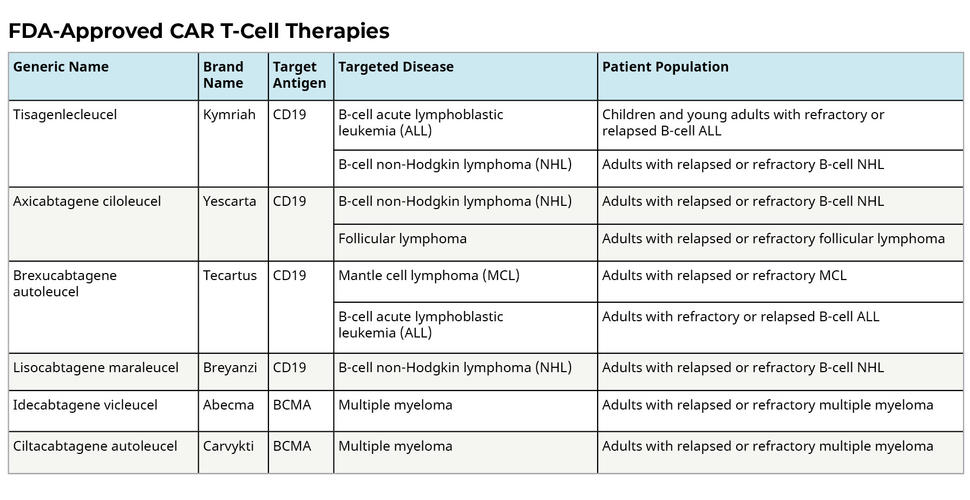
\includegraphics[width=1.0\columnwidth]{img/FDA Approved CAR T-Cell Therapies Table.jpeg}
    \end{center}
    \caption[Farmaci CAR-T approvati dall’FDA]{Farmaci CAR-T approvati dall’FDA
    \cite{img22}}

\end{figure}

Nel caso del LNH, il Tisagenlecleucel è indicato per i linfomi diffusi a grandi cellule B (DLBCL) recidivanti o 
refrattari dopo due linee di chemioterapia sistemica. L’ Axicabtageneciloleucel è stato approvato per linfomi 
diffusi a grandi cellule B (DLBCL) e linfoma a grandi cellule B primitivo del mediastino, 
refrattari o recidivanti, dopo due linee di chemioterapia sistemica\cite{EMATOCART}.\\
Il CAR è un recettore transmembrana chimerico, che, mediante l’utilizzo di vettori retrovirali o lentivirali, 
va a sostituire il TCR del linfocita.  
La terapia delle CAR-T è autologa, in quanto usa le cellule T proprie del paziente. La loro produzione sfrutta 
il processo di ingegnerizzazione.\\

La prima fase del processo di produzione delle CAR-T è la leucoaferesi, in cui viene prelevato il sangue dal 
paziente tramite una vena periferica; grazie al processo di aferesi il sangue prelevato viene separato in 
globuli rossi, globuli bianchi, piastrine e plasma, ma solo le cellule T dei globuli bianchi vengono prelevate, 
mentre il resto del sangue viene reinfuso al paziente. È una fase molto importante e delicata in quanto una bassa 
resa aferetica, provoca una ridotta espansione delle cellule CAR-T in vitro; questo può dipendere da una bassa conta 
leucocitaria, dalla presenza di numerose cellule natural killer (NK) e blasti nel sangue periferico\cite{EMATOCART},\cite{LLSCART}.\\
La seconda fase del processo prevede che le cellule T raccolte siano inviate a laboratori specializzati per la fase 
di ingegnerizzazione genetica, secondo cui il DNA viene introdotto all’interno delle cellule, per produrre CAR, 
grazie ai quali le cellule T acquisiscono la capacità di attaccare le cellule cancerose\cite{EMATOCART},\cite{LLSCART}.\\
Nella terza fase, il numero di cellule raccolte viene moltiplicato in laboratorio e quando si ha il quantitativo 
necessario, vengono criopreservate e rinviate al centro o all’ospedale dove il paziente le riceverà. 
Questo processo dura dalle tre alle quattro settimane.\\
Prima della somministrazione, il paziente, a partire da una settimana fino a due giorni prima, viene sottoposto 
alla chemioterapia di linfodeplezione che  serve a ridurre le cellule T normali nel corpo, per “fare spazio” alle 
cellule CAR-T ed avere una maggiore espansione in vivo.\\ 
Lo schema terapeutico maggiormente utilizzato prevede la somministrazione di ciclofosfamide e fludarabina.
L’ultima fase è di somministrazione del farmaco, previo scongelamento, in una via endovenosa centrale, 
della durata di circa trenta minuti\cite{EMATOCART}.\\
I centri autorizzati alla somministrazione delle CAR-T sono presenti in tutta Italia, in Toscana abbiamo 
i centri di Firenze e Pisa\cite{AILCENTRI}.\\

\begin{figure}[h]
    \begin{center}
    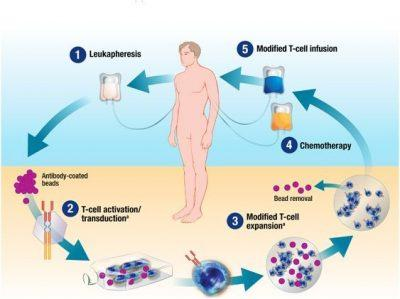
\includegraphics[width=1.0\columnwidth]{img/car-t process.jpeg}
    \end{center}
    \caption[Processo di costituzione e somministrazione delle CAR-T]{Processo di costituzione e somministrazione delle CAR-T
    \cite{img23}}

\end{figure}

\begin{figure}[h]
    \begin{center}
    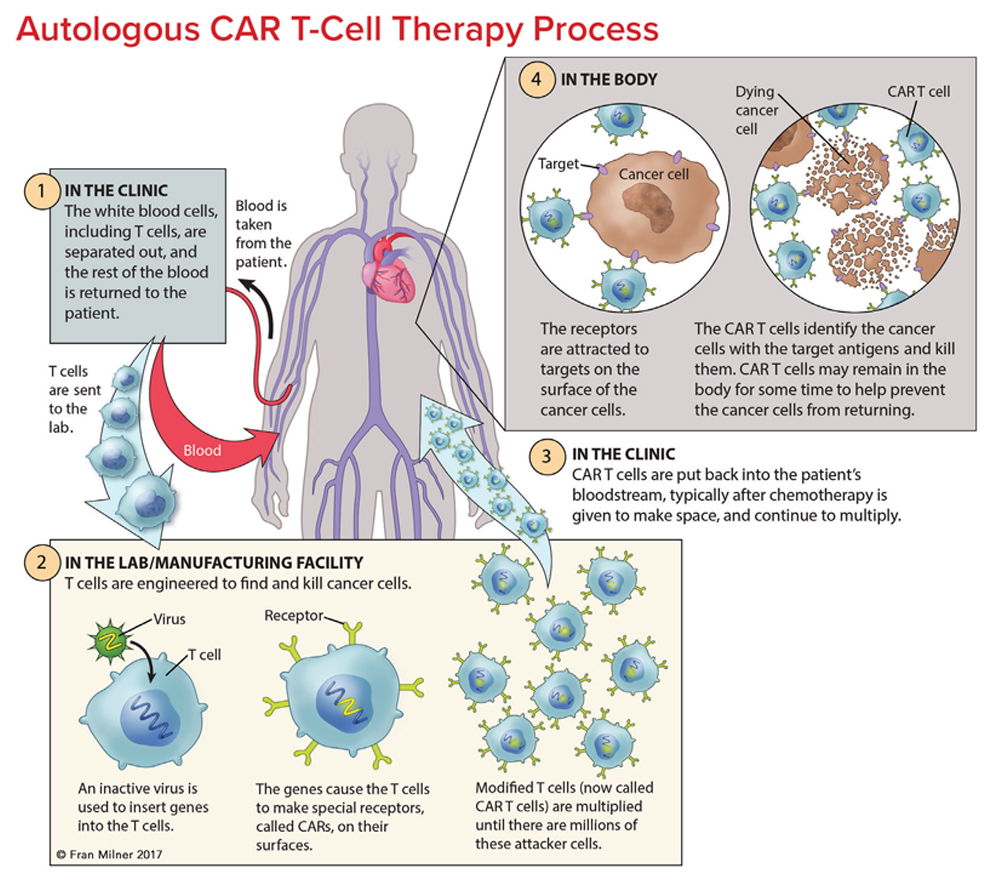
\includegraphics[width=1.0\columnwidth]{img/CART_TherapyProcess_Oct2020.jpeg}
    \end{center}
    \caption[Processo di prelievo, costituzione e somministrazione delle CAR-T]{Processo di prelievo, costituzione e somministrazione delle CAR-T
    \cite{img24}}

\end{figure}

Nonostante i risultati positivi dati dalla terapia delle CAR-T, che dimostrano il raggiungimento di risposte rapide e 
durature nel tempo, non mancano aspetti di tossicità acuta, che possono evolvere in situazioni di severità, se non 
anche di fatalità\cite{EMATOCART}.\\
La tossicità autoimmune si verifica quando il linfocita CAR-T riconosce come antigene target il CD-19 non solo nelle 
cellule cancerose, ma anche nelle cellule sane.
Il fenomeno è noto come “on-target-of-tissue effects”. È un effetto avverso che può risultare anche fatale.
È ciò che succede ai linfociti B sani, che presentano sulla loro superficie il target del linfocita CAR-T e vanno 
incontro ad aplasia. La ricerca, dovrebbe orientarsi a trovare una soluzione affinchè il target delle cellule CAR-T 
siano le cellule cancerose e non quelle sane\cite{Frontiers}.\\

Più frequentemente si assiste ad una sindrome da rilascio di citochine (CRS), che può manifestarsi con sintomi come 
astenia, febbre, mal di testa, tachicardia, ipotensione e ipossia, sintomi sistemici quali arresto cardiaco, aritmia, 
encefalopatia, insufficienza renale, fino ad arrivare ad una insufficienza multiorgano. La CRS può inoltre evolvere 
in una MAS (sindrome da attivazione macrofagica). 
La CRS può insorgere a partire da alcune ore, fino anche ad una settimana dalla somministrazione di CAR-T.\\
Diversi sono i fattori di rischio che comportano il manifestarsi di tale sintomatologia (immagine n. 25) che 
influiscono anche sul suo grado di severità; ad esempio un’ infusione di una dose elevata di CAR-T, le caratteristiche 
del paziente, il tipo di terapia di linfodeplezione, lo stato della malattia e il  burden di malattia 
(burden of disease), che dà una stima dell’impatto della malattia in termini di disabilità e mortalità\cite{EMATOCART}.\\

\begin{figure}[h]
    \begin{center}
    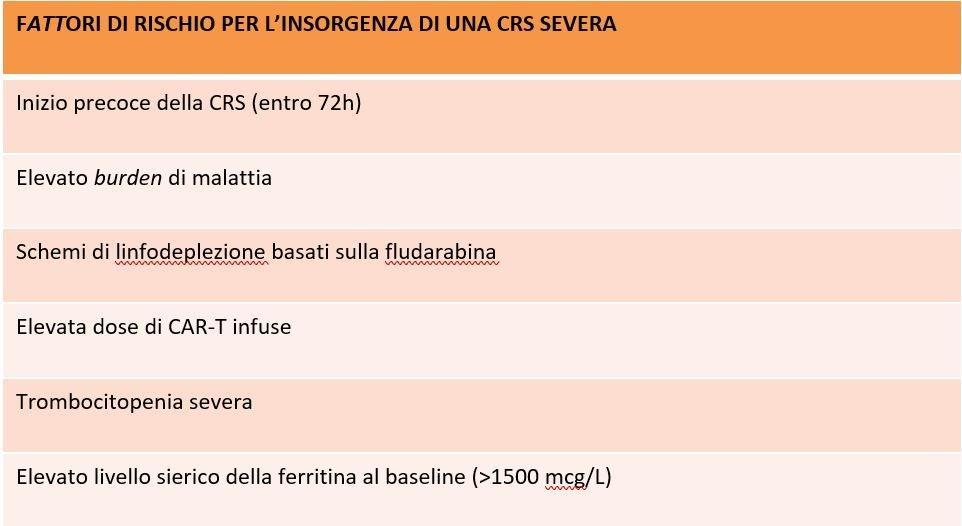
\includegraphics[width=1.0\columnwidth]{img/rischio CRS.jpeg}
    \end{center}
    \caption[Fattori di rischio per l’insorgenza di una CRS severa. ]{Fattori di rischio per l’insorgenza di una CRS severa. 
    \cite{img25}}

\end{figure}

Il grado di severità con cui si sviluppa la CRS è correlato agli elevati livelli ematici di CAR-T ed elevati livelli 
sierici di IL-6 (interleuchina-6); pertanto il trattamento di prima scelta della CRS moderata-severa, 
prevede la somministrazione di tocilizumab, un anticorpo monoclonale anti-IL-6\cite{EMATOCART}.\\
L’uso di corticosteroidi per la CRS, era precedentemente limitato, ma secondo studi più recenti il loro utilizzo 
non compromette l'attività delle CAR-T e l’outcome del paziente\cite{Cortico}.\\
Per valutare il grado di severità della CRS, l’ASTCT (American Society for Transplantation and Cellular Therapy) 
ha prodotto delle linee guida, secondo quanto riportato da \cite{ASTCT}.\\














